\termi{yhtälö}{Yhtälö} on väite kahden lausekkeen yhtäsuuruudesta.

\begin{esimerkki}
	\alakohdat{
		§ $x+3=\frac{5}{7}+2$ on yhtälö, joka väittää lausekkeiden $x+3$ ja $\frac{5}{7}+2$ olevan lukuarvoltaan yhtä suuret.
		§ $2=\frac{4}{2}$ on yhtälö, joka väittää, että luku $2$ voidaan esittää myös muodossa $\frac{4}{2}$.
	}
\end{esimerkki}

\laatikko{
	Jos yhtälön kummankin puolen lausekkeen arvo on sama, sanotaan että \termi{yhtälön päteminen}{yhtälö pätee} tai että yhtälö on tosi.
}

\begin{esimerkki}
	\alakohdat{
		§ Yhtälö $5=3$ ei päde.
		§ Yhtälö $t=t$ on tosi kaikilla muuttujan $t$ lukuarvoilla, sillä jokainen luku on varmasti yhtä suuri itsensä kanssa.
		§ Yhtälö $x=x+1$ on epätosi kaikilla $x$:n arvoilla, koska mikään luku ei voi olla yhtä suuri kuin sitä yhtä suurempi luku.
		§ Yhtälö $x+2=0$ pätee vain siinä tapauksessa, että $x=-2$.
	}
\end{esimerkki}

%yhtä suuri ERIKSEEN, ei yhdyssana


%Virkerakenne ja yhtälöiden luokittelulaatikon otsikointi\ldots
\laatikko[Yhtälöiden luokittelu]{
	\begin{description}
		\item[Aina tosi yhtälö] Esimerkiksi yhtälöt $8=8$ ja $x=x$
		\item[Joskus tosi yhtälö] Esimerkiksi yhtälö $x+4=7$ on tosi, kun $x=3$, ja epätosi muulloin.
		\item[Ei koskaan tosi yhtälö] Esimerkiksi yhtälö $0=1$
	\end{description}
}

Matematiikan sovelluksissa näistä tärkeimpiä ovat joskus (eli ehdollisesti) todet yhtälöt.

\laatikko[Yhtälöihin liittyviä käsitteitä]{
	\begin{description}
		\item[Tuntematon] Luku, jonka arvoa ei tiedetä. Tuntemattomia merkitään vaihtelevilla symboleilla. Jos tuntemattomia on vain yksi, sitä merkitään 	yleensä kirjaimella $x$ (alunperin kreikkalainen $\chi$, \textit{khi}).
		\item[Yhtälön ratkaisu(t)] Muuttujan arvo(t), jolla yhtälö pätee. Kutsutaan myös yhtälön juuriksi. (Nimityksellä ei ole mitään tekemistä juurenottolaskutoimituksen kanssa.)
		\item[Yhtälön ratkaiseminen] Kaikkien yhtälön ratkaisujen selvittäminen.
	\end{description}
}
Huomioi, että yhtälössä voi olla useitakin eri tuntemattomia. Kaikki kirjaimet eivät myöskään ole välttämättä tuntemattomia, vaan niillä voidaan tarkoittaa myös vakioita eli muuttumattomia lukuarvoja. Esimerkiksi fysiikassa käytetään usein eri kirjaimia merkitsemään eri luonnonvakioita.

\begin{esimerkki}
Tarkastellaan legendaarista fysiikan yhtälöä $E=mc^2$. Tässä yhtälössä on vakio $c$ eli valonnopeus, joka on luonnonvakio eikä siis (nykytiedon mukaan) muutu. Lisäksi yhtälössä on muuttujat $E$ eli energia ja $m$ eli massa. Riippuu käsiteltävästä tilanteesta, ovatko energia ja massa vakioita vai muuttujia, ja tuntemattomana voi eri tilanteessa toimia mikä tahansa: $E$, $m$ tai $c$.
\end{esimerkki}

\laatikko[Yhtälön muokkaaminen]{

Koska yhtälön puolet ovat yhtä suuret, eli tarkoittavat täsmälleen samaa asiaa, niin jonkin yhtälön molemmille puolille tehdyn laskutoimituksen jälkeen ne ovat edelleen yhtä suuret.
}

%selitetään, mitä on puolittain kertominen jne., puolittain\ldots\ldots


\begin{esimerkki}
%Lisännyt Jaakko Viertiö 2013-11-10
	\luettelo{
		§ Yhtälö $3x-12=6(\frac{1}{2x-2})$ on yhtäpitävä yhtälön $0=0$ kanssa, sillä se saadaan tähän muotoon 
		tekemällä yhtäpitävyyden molemmille puolille aina samat laskutoimitukset. Yhtälön yksinkertaisemmasta esityksestä $0=0$ nähdään, että muuttujan $x$ arvo ei vaikuta yhtälön ratkaisuihin. Toisin sanoen puolet ovat aina samat, olipa muuttuja $x$ mikä tahansa luku. Yhtälö on siis aina tosi.
		§ Yhtälö $3x-11=6(\frac{1}{2x-2})$ on yhtäpitävä yhtälön $0=1$ kanssa. Jälkimmäisestä muodosta nähdään, ettei yhtälö voi olla tosi millään muuttujan $x$ arvolla, sillä yhtälön muodossa $0=1$ ei esiinny muuttujaa $x$. Täten $x$ ei vaikuta yhtälön ratkaisuihin. Yhtälö on siis aina epätosi.
		§ Yhtälö $3x-11=6(x-2)$ on yhtäpitävä yhtälön $x=\frac{1}{3}$ kanssa. Yhtälö on siis joskus tosi: täsmälleen silloin kun $x=\frac{1}{3}$. Tämä voidaan tarkistaa sijoittamalla yhtälöön $x$:n paikalle arvo $\frac{1}{3}$, jolloin yhtälön vasen ja oikea puoli ovat yhtä suuret.
	}

\end{esimerkki}

%esimerkki yhtälön ratkaisun tarkistamisesta!
%Esimerkki yhtälöstä, jolla on useita ratkaisuja! annettujen juuriehdotusten tarkistaminen
%esimerkki, että yhtälön ratkaisun voi myös arvata!


%yhtälöpariesimerkki, viittaus transitiivisuuteen

Yhtälöitä käyttämällä voidaan mallintaa monia käytännön tilanteita.

\begin{esimerkki}
	Yksinkertainen esimerkki yhtälön käyttämisestä on matkaan kuluvan ajan ratkaiseminen matkan pituuden ja nopeuden avulla. Kuljettu matka on nopeus kerrottuna kuljetulla ajalla. 
	
	Jos matka on 15 kilometriä ja nopeus 5 km/h, voimme merkitä $5\cdot t=15$, jossa $t$ on matkaan kuluvaa aikaa kuvaava \termi{muuttuja}{muuttuja}.
\end{esimerkki}

Toisaalta yhtälöjä voidaan käyttää myös abstraktimpien pulmien ratkaisuun.

\begin{esimerkki}
	Halutaan tietää, onko olemassa lukua, jonka kolmas potenssi jaettuna kolmella on yhtä suuri kuin sen toinen potenssi jaettuna kahdella. Tällöin merkitään $\frac{x^3}{3}=\frac{x^2}{2}$. 
\end{esimerkki}
	%%\begin{esimerkki}
%%	Merkitään lausekkeet $5x+\sqrt{x}$ ja $7x+7$ yhtäsuuriksi, jolloin saadaan yhtälö $5x+\sqrt{x} = 7x+7$.
%%\end{esimerkki}


%Lisännyt Jaakko Viertiö 2013-11-10
\begin{esimerkki}
Tarkastellaan yhtälöä $x^3-2x^2-x+2=0$.  Yhtälössä on yksi muuttuja $x$ ja neljä termiä: $x^3$, $-2x^2$, $-x$ ja $+2$. Yhtälön \textit{eräs} ratkaisu on $x=1$, sillä $1^3-2\cdot{1^2}-1+2=0$. Myös $x=2$ on kyseisen yhtälön ratkaisu, sillä $2^3-2\cdot{2^2}-2+2=0$. Tuntemattomalle $x$ voidaan siis joissain tapauksissa löytää useita arvoja, jotka toteuttavat yhtälön. 
\end{esimerkki}

\subsection*{Yhtälön ratkaiseminen}

Tyypillinen tapa ratkaista yhtälöitä on kirjoittaa ne ilmaistuna toisella tavalla. Käytännössä tämä tarkoittaa niiden muokkaamista siten, ettei alkuperäisen yhtälön paikkansapitävyys muutu. Tällä tavalla saadaan eri yhtälö, jolla on kuitenkin samat ratkaisut. Yleensä tavoitteena on saada yhtälö muotoon, jossa yhtäpitävyyden toisella puolella on vain haluttu muuttuja ilman kertoimia ja toisella puolella kaikki muu.  Yhtälön ratkaisemiseksi näitä muunnoksia toistetaan, kunnes yhtälön ratkaisu on helposti luettavissa.

\begin{esimerkki}
Ratkaistaan aiemman esimerkin matkan kesto. Yhtälö on siis $5t=15$, jossa $t$ on aika, nopeus on $5$\,km/h ja matkan pituus $15$\,km. Jakamalla laskusääntöjen mukaan yhtälön molemmat puolet viidellä, saadaan yhtälö muotoon $t=3$, joka on samalla kyseisen yhtälön ratkaisu.
\end{esimerkki}

%HELPOMPI ESIMERKKI, JA TÄÄ MUUTENKIN TURHAN VAIKEA AINEEN JA PIINEEN :)
\begin{esimerkki}
Ratkaistaan yhtälö $\frac{4\sqrt{x}a}{3}=8a$, jossa $a$ on vakio $\pi$ eli yhtälö voidaan kirjoittaa muotoon $\frac{4\pi\sqrt{x}}{3}=8\pi$.

		\begin{align*}
			\frac{4 \pi \sqrt{x}}{3} &= 8 {\pi} && \text{| Jaetaan molemmat puolet luvulla $\frac{4}{3}$.} \\
			{\pi}\sqrt{x} &= \frac{8\cdot 3\cdot {\pi}}{4} && \text{| Jaetaan molemmat puolet luvulla $\pi$.} \\
			\sqrt{x} &= \frac{24}{4} && \text{| Sievennellään.} \\
			\sqrt{x} &= 6 && \text{| Tässä huomataan, että $\sqrt{36}=6$.} \\
\end{align*}

Joten yhtälöllä on ratkaisu $x=36$.

\end{esimerkki}

Yhtälön ratkaisemista voidaan ajatella havainnollisemmin kuvittelemalla orsivaaka, joka on tasapainossa. Vasemmalla ja oikealla puolella on eripainoisia esineitä, mutta ne painavat yhteensä yhtä paljon. Jos molemmille puolille lisätään nyt saman verran painoa, vaaka on yhä tasapainossa. Samalla tavalla yhtälön molemmille puolille on sallittua lisätä sama luku.

\begin{esimerkki}
Kuvassa oleva vaaka on tasapainossa. Toisessa vaakakupissa on kahden kilon siika ja toisessa puolen kilon ahven sekä tuntematon määrä lakritsia.	Kuinka paljon vaakakupissa on lakritsia?
	\begin{center}
		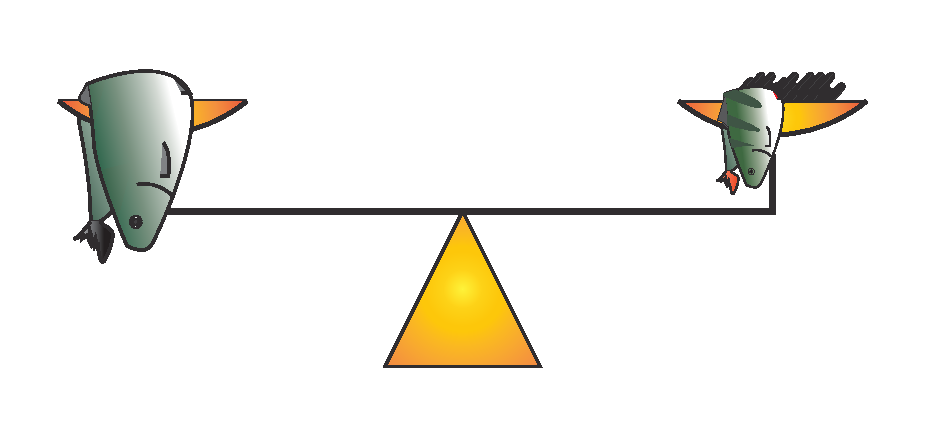
\includegraphics[scale=0.6]{pictures/Kuva10-1-vaaka.pdf} % CC-BY Lilja Tamminen
		%\includegraphics{unused/kala-vaaka.png} % CC-BY Hannu Köngäs
		% FIXME: Hannun piirros on viimeistellympi (smoothit värjäykset jne.), Liljan piirros taas konsistentimpi
		% kirjan muun kuvituksen kanssa. Kumpi jätetään? Nyt päällä Liljan kuva.
	\end{center}
	\begin{esimratk}
Merkitään lakritsin määrää tuntemattomalla $x$. Tilannetta kuvaa yhtälö $2 = 0,5 + x$, joka muodostetaan vaa'an toiminnan ymmäryksen avulla: tasapainossa molemmissa vaakakupeissa tulee olla massaltaan yhtä paljon ainetta, eli massat (määrät) voidaan merkitä yhtä suuriksi.

Ratkaistaan yhtälö.
		\begin{align*}
			2 &= 0,5 + x &&\text{| $-0,5$} \\
			2 - 0,5 &= x && \\
			1,5 &= x && \\
			x &= 1,5 &&
		\end{align*}
	\end{esimratk}
	\begin{esimvast}
		Lakritsia on $1,5$ kg.
	\end{esimvast}
\end{esimerkki}

\begin{esimerkki}
Juna Helsingistä Jyväskylään kulkee $342$ kilometrin matkan kolmessa tunnissa ja $23$ minuutissa tasaista vauhtia. $10$ minuuttia junan lähdön jälkeen auto lähtee Helsingistä Jyväskylään kulkien tasaista $100$ kilometrin tuntivauhtia. Jyväskylään on Helsingistä maanteitse $272$ kilometriä. Kuinka kauan auton lähdöstä on kulunut, kun juna ja auto ovat kulkeneet yhtä suuren osan omista matkoistaan?
	\begin{esimratk}
		Lasketaan aluksi junan nopeus
		\[3\,\text{h} \; 23\,\text{min} \; = 12\,180\,\text{s} \]
		\[\frac{342\,000\,\text{m}}{12\,180\,\text{s}} \approx  28,0788\,\frac{\text{m}}{\text{s}} \]
		%SIEVENNETYT MURTOLUVUT + HUOMAUTUS LIKIARVOISTA!
		Muunnetaan lisäksi auton nopeus yksikköön $\frac{\text{m}}{\text{s}}$ (muuntokerroin $3,6$).
		\[100\,\frac{\text{km}}{\text{h}} \approx 27,7778 \frac{\text{m}}{\text{s}} \]
		
		$10$ minuuttia on $600$ sekuntia.
		
		Voidaan nyt muotoilla yhtälö käyttäen yksiköitä metri ja sekunti. Tuntemattomaksi valitaan $t$, joka kuvaa aikaa sekunteina auton lähdöstä.
		\[ \frac{28,0788(t+600)}{342\,000} = \frac{27,7778t}{272\,000} \]
		
		Ratkaistaan yhtälö
		\begin{align*}
			\frac{27,7778t}{272\,000} &= \frac{28,0788(t+600)}{342\,000} &&\text{| $\cdot{272\,000}$} &&\text{| $\cdot{342\,000}$}  \\
			342\,000 \cdot 27,7778t &= 272\,000 \cdot 28,0788(t+600) \\
			9\,500\,007,6t &= 7\,637\,433,6(t+600) \\
			9\,500\,007,6t &= 7\,637\,433,6t + 4\,582\,460\,160 &&\text{| $-7\,637\,433,6t$} \\ 
			1\,862\,574t &= 4\,582\,460\,160 &&\text{| $:{1\,862\,574}$} \\
			t &\approx 2\,460,28 \approx 2\,460
		\end{align*}
		
		Muutetaan yksiköksi minuutit
		\[2\,460\,\text{s}=41\,\text{min}\]
	\end{esimratk}
	\begin{esimvast}
		$41$ minuuttia
	\end{esimvast}
\end{esimerkki}

Mitään varsinaista ei virhettä yhtälönratkaisussa ei ole tehty niin kauan kuin sama operaatio tehdään aina yhtälön molemmille puolille, mutta vaatii rutiinia, jotta oppii, mitä laskutoimituksia kannattaa tehdä ja missä järjestyksessä. Seuraavassa joitakin yleisiä toimenpiteitä yhtälöiden ratkaisuun, joita voi soveltaa päästäkseen eteenpäin. Kyseessä ei ole mikään aina toimiva ratkaisuohje, vaan yleisiä vinkkejä.

\laatikko[Yleisiä yhtälönratkaisuperiaatteita]{
	\begin{description}
		\item[1)] Kerro tuntematonta sisältävät lausekkeet pois nimittäjistä.
		\item[2)] Yhdistä useat murtolausekkeet yhdeksi laventamalla ne samannimisiksi.
		\item[3)] Siirrä tuntemattomia sisältävät yhtälön osat samalle puolelle ja ota tuntematon yhteiseksi tekijäksi.
		\item[4)] Kumoa juuret ja murtopotenssit korottamalla yhtälö puolittain sopivaan potenssiin.
		\item[5)] Sulkuja ei välttämättä aina kannata kertoa auki.
		\item[6)] Yhtälö on ratkaistu vasta, kun jäljellä on enää vain yksi kappale tuntematonta suuretta, ja se sijaitsee yksin omalla puolellaan yhtälöä.
	\end{description}
}

\section*{Yhtälöpari}

Joissakin tilanteissa ratkaistavana on useampi tuntematon. Kuitenkin yhdestä yhtälöstä voi ratkaista korkeintaan yhden tuntemattoman kerrallaan, joten ratkaistaessa kahta tuntematonta tarvitaan kaksi yhtälöä. Yleisesti:

\laatikko{Jos ratkaistaan $n$ tuntematonta, tähän tarvitaan vähintään $n$ toisistaan riippumatonta yhtälöä.}

Jos halutaan esimerkiksi selvittää, mitkä luvut $x$ ja $y$ toteuttavat sekä yhtälön $2x=y+5$ ja toisaalta 
myös yhtälön $x-10=4y+2$, ratkaistaan nämä molemmat niin sanottuna \termi{yhtälöpari}{yhtälöparina}. Yleensä samanaikaisesti ratkottavat yhtälöt merkitään allekain seuraavasti:
$$\left\{    
    \begin{array}{rcl}
        2x&=&y+5 \\
        x-10&=&4y+2 \\
    \end{array}
    \right.$$

Yleinen, aina toimiva ratkaisumenetelmä yhtälöpareille on ratkaista jommasta kummasta yhätlöstä erikseen toinen tuntematon ja sijoitetaan saatu ratkaisu toiseen yhtälöön, jolloin yksi \termi{tuntemattoman eliminointi}{tuntematon eliminoituu} eli poistuu, jolloin ongelma yksinkertaistuu yhden tuntemattoman ratkaisuksi.

\begin{esimerkki}
Ratkaise yhtälöpari $2x=y+5$; $x-10=4y+2$. Ratkaistaan molemmista yhtälöistä muuttuja $x$. 
	
	\begin{align*}
	    2x &= y+5 \\
	    x &= \frac{y+5}{2}
	\end{align*}
	\begin{align*}
	    x-10 &= 4y+2 \\
	    x &= 4y+12
	\end{align*}
	
Nyt yhtäsuuruusrelaation transitiivisuuden perusteella, koska $\frac{y+5}{2}=x$ ja toisaalta $x=4y+12$, saadaan yhtälö $\frac{y+5}{2}=4y+12$, joka osataan ratkaista.

\begin{align*}
	\frac{y+5}{2} &= 4y+12 \\
	y+5 &= 2(4y+12)\\
	y+5 &= 8y+24 \\
	y -8y&= 24-5 \\
	-7y &= 19 \\
	y=-\frac{19}{7}
\end{align*}

Nyt saatu $y$:n arvo voidaan sijoittaa jompaan kumpaan alkuperäiseen yhtälöön, esimerkiksi yhtälöön $2x=y+5$, ja tästä saadaan ratkaistua myös $x$.

\begin{align*}
      2x &= -\frac{19}{7}+5\\
      2x &= \frac{16}{7} \\
      x &= -\frac{8}{7}
\end{align*}

Siis yhtälöparin ratkaisu on $x=\frac{8}{7}$ ja $y=-\frac{19}{7}$. Sijoittamalla voidaan tarkistaa, että luvut todellakin toteuttavat molemmat alkuperäiset yhtälö..
\end{esimerkki} %TEHTÄVIÄ JA SOVELLUKSIA!

Yhtälöparien ja yhtälöryhmien ratkaisuun ja geometriseen merkitykseen tutustutaan tarkemmin MAA4-kurssilla.
